\documentclass[tikz]{standalone}
\usepackage{amsmath}
\usepackage{xcolor}
\definecolor{bg}{HTML}{171D2B}
\definecolor{aksen}{HTML}{F7B538}
\pagecolor{bg}
\color{white}
\usetikzlibrary{arrows.meta}
\begin{document}
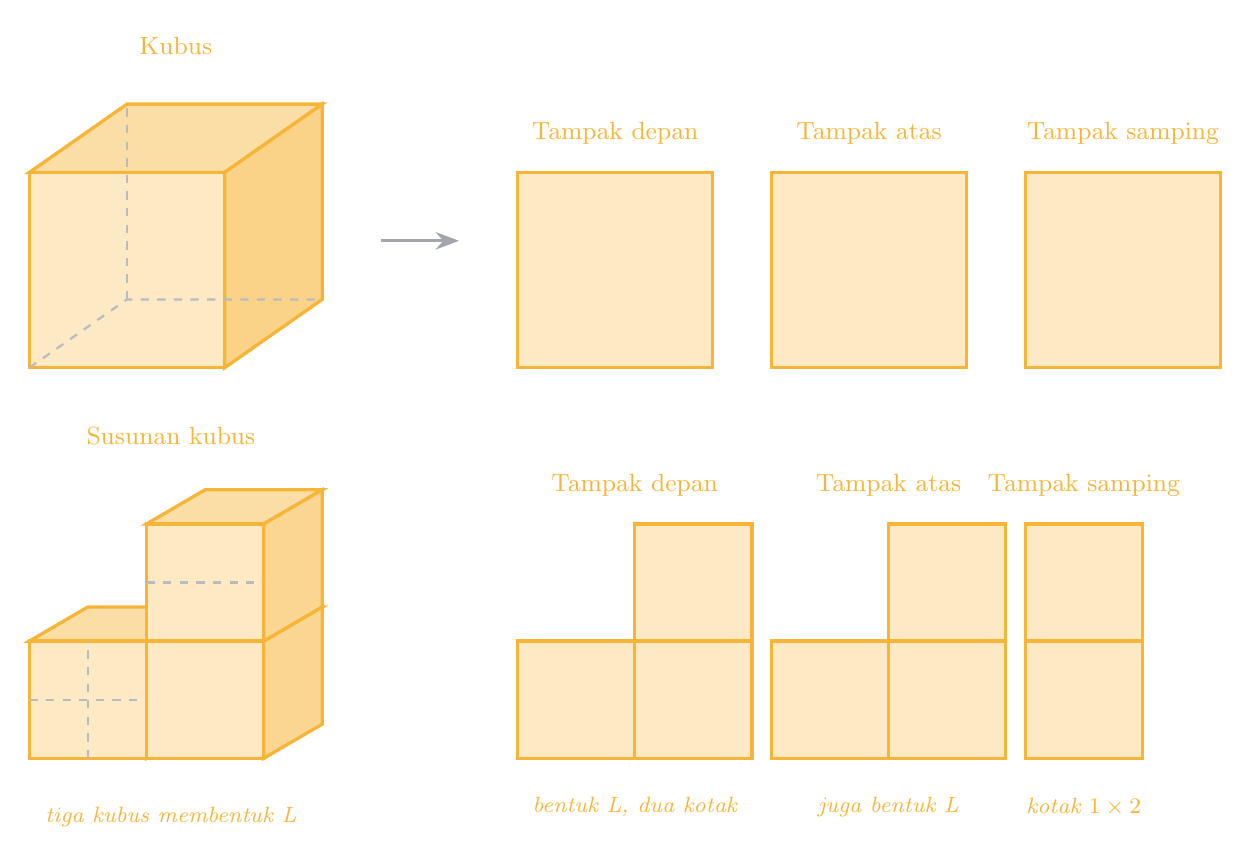
\begin{tikzpicture}[scale=0.62,>=Stealth,
  bangun/.style={draw=aksen,very thick},
  garisputih/.style={draw=white!70!bg,thick,dashed},
  label/.style={color=aksen,font=\small}]

  % ---------- Kubus 3D (proyeksi kabinet) ----------
  \begin{scope}[shift={(0,0)}]
    \coordinate (A) at (0,0);
    \coordinate (B) at (4,0);
    \coordinate (C) at (4,4);
    \coordinate (D) at (0,4);
    \coordinate (A2) at (2,1.4);
    \coordinate (B2) at (6,1.4);
    \coordinate (C2) at (6,5.4);
    \coordinate (D2) at (2,5.4);
    \draw[bangun,fill=aksen!45] (D) -- (C) -- (C2) -- (D2) -- cycle;   % atas
    \draw[bangun,fill=aksen!60] (B) -- (C) -- (C2) -- (B2) -- cycle;   % kanan
    \draw[bangun,fill=aksen!30] (A) -- (B) -- (C) -- (D) -- cycle;     % depan
    \draw[garisputih] (A) -- (A2) -- (B2);
    \draw[garisputih] (A2) -- (D2);
    \node[label] at (3,6.6) {Kubus};
  \end{scope}

  \draw[->,very thick,white!60!bg] (7.2,2.6) -- (8.8,2.6);

  % ---------- Tampak depan ----------
  \begin{scope}[shift={(10,0)}]
    \draw[bangun,fill=aksen!30] (0,0) rectangle (4,4);
    \node[label] at (2,4.8) {Tampak depan};
  \end{scope}

  % ---------- Tampak atas ----------
  \begin{scope}[shift={(15.2,0)}]
    \draw[bangun,fill=aksen!30] (0,0) rectangle (4,4);
    \node[label] at (2,4.8) {Tampak atas};
  \end{scope}

  % ---------- Tampak samping ----------
  \begin{scope}[shift={(20.4,0)}]
    \draw[bangun,fill=aksen!30] (0,0) rectangle (4,4);
    \node[label] at (2,4.8) {Tampak samping};
  \end{scope}

  % ---------- Pola susunan kubus: depan = persegi, atas = L ----------
  \begin{scope}[shift={(0,-8)}]
    \node[label] at (2.9,6.6) {Susunan kubus};
    % susunan L: dua kubus alas + satu kubus di atas kanan (proyeksi kabinet, kedalaman +1.2,+0.7)
    \def\dx{1.2} \def\dy{0.7}
    % kubus kiri-bawah
    \draw[bangun,fill=aksen!45] (0,2.4) -- (\dx,3.1) -- (2.4+\dx,3.1) -- (2.4,2.4) -- cycle;
    \draw[bangun,fill=aksen!55] (2.4,0) -- (2.4+\dx,\dy) -- (2.4+\dx,2.4+\dy) -- (2.4,2.4) -- cycle;
    \draw[bangun,fill=aksen!30] (0,0) rectangle (2.4,2.4);
    \draw[garisputih] (0,1.2) -- (2.4,1.2);
    \draw[garisputih] (1.2,0) -- (1.2,2.4);
    % kubus kanan-bawah
    \draw[bangun,fill=aksen!45] (2.4,2.4) -- (2.4+\dx,3.1) -- (4.8+\dx,3.1) -- (4.8,2.4) -- cycle;
    \draw[bangun,fill=aksen!55] (4.8,0) -- (4.8+\dx,\dy) -- (4.8+\dx,2.4+\dy) -- (4.8,2.4) -- cycle;
    \draw[bangun,fill=aksen!30] (2.4,0) rectangle (4.8,2.4);
    % kubus kanan-atas
    \draw[bangun,fill=aksen!45] (2.4,4.8) -- (2.4+\dx,5.5) -- (4.8+\dx,5.5) -- (4.8,4.8) -- cycle;
    \draw[bangun,fill=aksen!55] (4.8,2.4) -- (4.8+\dx,3.1) -- (4.8+\dx,4.8+\dy) -- (4.8,4.8) -- cycle;
    \draw[bangun,fill=aksen!30] (2.4,2.4) rectangle (4.8,4.8);
    \draw[garisputih] (2.4,3.6) -- (4.8,3.6);
    \node[label,font=\footnotesize\itshape] at (2.9,-1.2) {tiga kubus membentuk L};
  \end{scope}

  \begin{scope}[shift={(10,-8)}]
    \draw[bangun,fill=aksen!30] (0,0) rectangle (2.4,2.4);
    \draw[bangun,fill=aksen!30] (2.4,0) rectangle (4.8,2.4);
    \draw[bangun,fill=aksen!30] (2.4,2.4) rectangle (4.8,4.8);
    \node[label] at (2.4,5.6) {Tampak depan};
    \node[label,font=\footnotesize\itshape] at (2.4,-1.0) {bentuk L, dua kotak};
  \end{scope}

  \begin{scope}[shift={(15.2,-8)}]
    \draw[bangun,fill=aksen!30] (0,0) rectangle (2.4,2.4);
    \draw[bangun,fill=aksen!30] (2.4,0) rectangle (4.8,2.4);
    \draw[bangun,fill=aksen!30] (2.4,2.4) rectangle (4.8,4.8);
    \node[label] at (2.4,5.6) {Tampak atas};
    \node[label,font=\footnotesize\itshape] at (2.4,-1.0) {juga bentuk L};
  \end{scope}

  \begin{scope}[shift={(20.4,-8)}]
    \draw[bangun,fill=aksen!30] (0,0) rectangle (2.4,2.4);
    \draw[bangun,fill=aksen!30] (0,2.4) rectangle (2.4,4.8);
    \node[label] at (1.2,5.6) {Tampak samping};
    \node[label,font=\footnotesize\itshape] at (1.2,-1.0) {kotak $1\times 2$};
  \end{scope}
\end{tikzpicture}
\end{document}
